\reviewexercisesheader{}

% 35

\eoce{% Replaces gpa_study_hours
\qt{Pet names\label{seattle_pet_names}}
The city of Seattle, WA has an open data portal that
includes pets registered in the city.
For each registered pet,
we have information on the pet's name and species.
The following visualization plots the proportion of dogs
with a given name versus the proportion of cats with the
same name.
The 20 most common cat and dog names are displayed.
The diagonal line on the plot is the $x = y$ line;
if a name appeared on this line, the name's popularity
would be exactly the same for dogs and cats.

\noindent\begin{minipage}[c]{0.4\textwidth}
\raggedright\begin{parts}
\item
    Are these data collected as part of an experiment
    or an observational study?
\item
    What is the most common dog name? What is the most
    common cat name?
\item
    What names are more common for cats than dogs?
\item
    Is the relationship between the two variables
    positive or negative? 
    What does this mean in context of the data?
\end{parts}\vspace{5mm}
\end{minipage}
\begin{minipage}[c]{0.05\textwidth}
\ 
\end{minipage}
\begin{minipage}[c]{0.53\textwidth}
\begin{center}
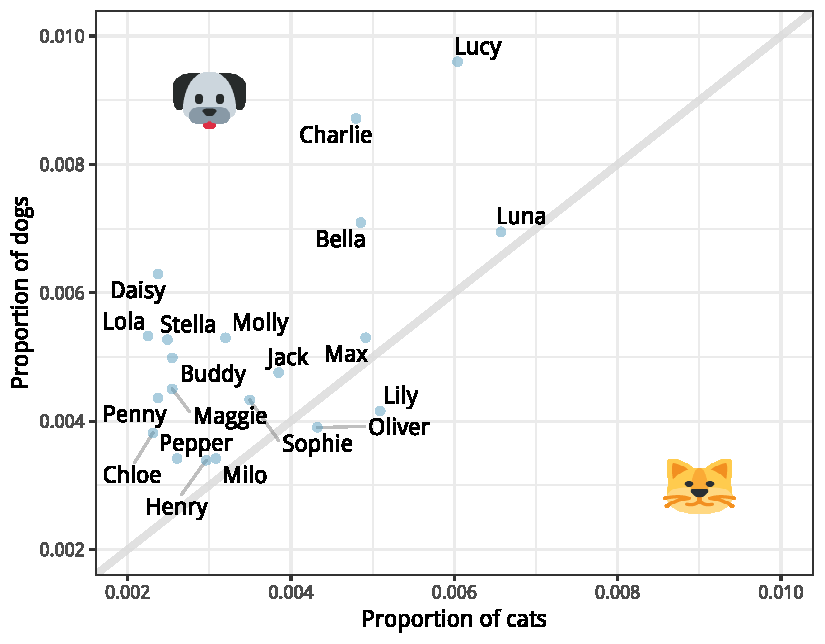
\includegraphics[width = 0.95\textwidth]{ch_data_collection/figures/eoce/seattle_pet_names/seattle_pet_names.pdf}
\end{center}
\end{minipage}
}{}

% 36

\eoce{\qt{Stressed out, Part II\label{stressed_out_experiment}} In a study evaluating the 
relationship between stress and muscle cramps, half the subjects are randomly assigned to be exposed to increased stress by being placed into an elevator that falls rapidly and stops abruptly and the other half are left at no or baseline stress.
\begin{parts}
\item What type of study is this?
\item Can this study be used to conclude a causal relationship between increased stress 
and muscle cramps?
\end{parts}
}{}

% 37

\eoce{\qt{Chia seeds and weight loss\label{chia_weight_lostt}} Chia Pets -- those terra-cotta 
figurines that sprout fuzzy green hair -- made the chia plant a household name. But chia 
has gained an entirely new reputation as a diet supplement.  In one 2009 study, a team 
of researchers recruited 38 men and divided them randomly into two groups: treatment or 
control. They also recruited 38 women, and they randomly placed half of these 
participants into the treatment group and the other half into the control group. One 
group was given 25 grams of chia seeds twice a day, and the other was given a placebo. 
The subjects volunteered to be a part of the study. After 12 weeks, the scientists found 
no significant difference between the groups in appetite or weight loss. 
\footfullcite{Nieman:2009}
\begin{parts}
\item What type of study is this? 
\item What are the experimental and control treatments in this study?
\item Has blocking been used in this study? If so, what is the blocking variable?
\item Has blinding been used in this study?
\item Comment on whether or not we can make a causal statement, and indicate whether or 
not we can generalize the conclusion to the population at large.
\end{parts}
}{}

% 38

\eoce{\qt{City council survey\label{city_council_survey}}
A city council has requested a household survey be conducted
in a suburban area of their city.
The area is broken into many distinct and unique neighborhoods,
some including large homes, some with only apartments, and others
a diverse mixture of housing structures.
For each part below,
identify the sampling methods described,
and describe the statistical pros and cons of the method
in the city's context.
\begin{parts}
\item
    Randomly sample 200 households from the city.
\item
    Divide the city into 20 neighborhoods,
    and sample 10 households from each neighborhood.
\item
    Divide the city into 20 neighborhoods,
    randomly sample 3 neighborhoods,
    and then sample all households from those 3 neighborhoods.
\item
    Divide the city into 20 neighborhoods,
    randomly sample 8 neighborhoods,
    and then randomly sample 50 households
    from those neighborhoods.
\item
    Sample the 200 households closest to the city council offices.
\end{parts}
}{}

\D{\newpage}

%39

\eoce{\qt{Flawed reasoning\label{flawed_reasoning}} Identify the flaw(s) in reasoning 
in the following scenarios. Explain what the individuals in the study should 
have done differently if they wanted to make such strong conclusions.
\begin{parts}
\item Students at an elementary school are given a questionnaire that they 
are asked to return after their parents have completed it. One of the questions 
asked is, ``Do you find that your work schedule makes it difficult for you to 
spend time with your kids after school?" Of the parents who replied, 85\% said 
``no". Based on these results, the school officials conclude that a great 
majority of the parents have no difficulty spending time with their kids 
after school.
\item A survey is conducted on a simple random sample of 1,000 women who 
recently gave birth, asking them about whether or not they smoked during 
pregnancy. A follow-up survey asking if the children have respiratory problems 
is conducted 3 years later, however, only 567 of these women are reached at the 
same address. The researcher reports that these 567 women are representative 
of all mothers.
\item An orthopedist administers a questionnaire to 30 of his patients who do 
not have any joint problems and finds that 20 of them regularly go running. 
He concludes that running decreases the risk of joint problems.
\end{parts}
}{}

% 40

\eoce{\qt{Income and education in US counties\label{income_education_county}} 
The scatterplot below shows the relationship between per capita income 
(in thousands of dollars) and percent of population with a bachelor's 
degree in 3,142 counties in the US using American Community Survey data from 2017.

\noindent\begin{minipage}[c]{0.44\textwidth}
\begin{parts}
\item What are the explanatory and response variables?
\item Describe the relationship between the two variables. Make sure to discuss 
unusual observations, if any.
\item Can we conclude that having a bachelor's degree increases one's income?
\end{parts}\vspace{8mm}
\end{minipage}
\begin{minipage}[c]{0.55\textwidth}
\begin{center}
\href{\oiRedirectUrl{tableau-scatter-income-bachelors}}{
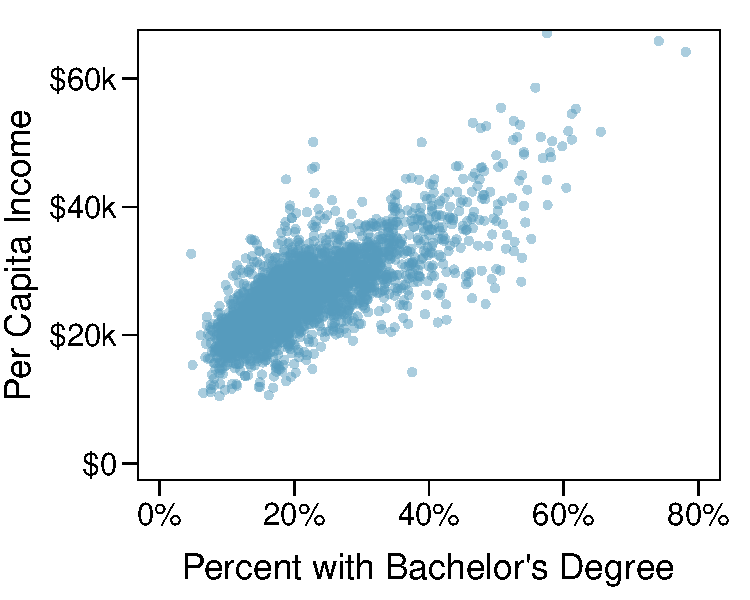
\includegraphics[width = 0.78\textwidth]{ch_data_collection/figures/eoce/county_income_education/county_income_education_scatterplot.pdf}
}
\tableauhref{tableau-scatter-income-bachelors}
\end{center}
\end{minipage}
}{}

% 41

\eoce{\qt[?]{Eat better, feel better\label{eat_better_feel_better}}
In a public health 
study on the effects of consumption of fruits and vegetables on psychological 
well-being in young adults, participants were randomly assigned to three 
groups: (1) diet-as-usual, (2) an ecological momentary intervention involving 
text message reminders to increase their fruits and vegetable consumption plus 
a voucher to purchase them, or (3) a fruit and vegetable intervention in 
which participants were given two additional daily servings of fresh fruits and 
vegetables to consume on top of their normal diet. Participants were asked to 
take a nightly survey on their smartphones.
Participants were student volunteers at the University of 
Otago, New Zealand.
At the end of the 14-day study, only participants in the third
group showed improvements to their psychological well-being across
the 14-days relative to the other groups.\footfullcite{conner2017let}
\begin{parts}
\item
    What type of study is this?
\item
    Identify the explanatory and response variables.
\item
    Comment on whether the results of the study can be generalized to
    the population.
\item
    Comment on whether the results of the study can be used to establish
    causal relationships.
\item
    A newspaper article reporting on the study states,
    ``The results of this study provide proof that giving young adults
    fresh fruits and vegetables to eat can have psychological benefits,
    even over a brief period of time.''
    How would you suggest revising this statement so that it can be
    supported by the study?
\end{parts}
}{}

\D{\newpage}

% 42

\eoce{\qt{Screens, teens, and psychological well-being\label{screen_time_well_being}}
In a study of three nationally representative large-scale data sets from Ireland, 
the United States, and the United Kingdom (n = 17,247), teenagers between the 
ages of 12 to 15 were asked to keep a diary of their screen time and answer questions about how they felt or acted.
The answers to these questions 
were then used to compute a psychological well-being score.
Additional data were collected and included in the analysis,
such as each child's sex and age, and on the mother’s education,
ethnicity, psychological distress, and employment.
The study concluded that there is little clear-cut evidence
that screen time decreases adolescent
well-being.\footfullcite{orben2018screens}
\begin{parts}
\item
    What type of study is this?
\item
    Identify the explanatory variables.
\item
    Identify the response variable.
\item
    Comment on whether the results of the study can be generalized
    to the population, and why.
\item
    Comment on whether the results of the study can be used
    to establish causal relationships.
\end{parts}
}{}

% 43

\eoce{\qt{Stanford Open Policing\label{stanford_open_policing}}
The Stanford Open Policing project gathers, analyzes, and
releases records from traffic stops by law enforcement 
agencies across the United States.
Their goal is to help researchers, journalists, and policymakers
investigate and improve interactions between police and the
public.\footfullcite{pierson2017large}
The following is an excerpt from a summary table created based off of the data 
collected as part of this project.
\begin{center}
\begin{tabular}{lllrrr}
\hline
               &           & Driver's  & No. of stops & \multicolumn{2}{c}{\% of stopped}  \\
County         & State     & race      & per year     & cars searched & drivers arrested \\ 
\hline
Apaice County  & Arizona   & Black     & 266          & 0.08          & 0.02 \\ 
Apaice County  & Arizona   & Hispanic  & 1008         & 0.05          & 0.02 \\ 
Apaice County  & Arizona   & White     & 6322         & 0.02          & 0.01 \\ 
Cochise County & Arizona   & Black     & 1169         & 0.05          & 0.01 \\ 
Cochise County & Arizona   & Hispanic  & 9453         & 0.04          & 0.01 \\ 
Cochise County & Arizona   & White     & 10826        & 0.02          & 0.01 \\ 
$\cdots$       & $\cdots$  & $\cdots$  & $\cdots$     & $\cdots$      & $\cdots$ \\
Wood County    & Wisconsin & Black     & 16           & 0.24          & 0.10 \\ 
Wood County    & Wisconsin & Hispanic  & 27           & 0.04          & 0.03 \\ 
Wood County    & Wisconsin & White     & 1157         & 0.03          & 0.03 \\ 
\hline 
\end{tabular}
\end{center}
\begin{parts}
\item
    What variables were collected on each individual traffic stop
    in order to create to the summary table above?
\item
    State whether each variable is numerical or categorical.
    If numerical, state whether it is continuous or discrete.
    If categorical, state whether it is ordinal or not.
\item
    Suppose we wanted to evaluate whether vehicle search rates
    are different for drivers of different races.
    In this analysis, which variable would be the response
    variable and which variable would be the explanatory variable?
\end{parts}
}{}

% 44

\eoce{\qt{Space launches\label{space_launches}}
The following summary table shows the number of space
launches in the US by the type of launching agency and
the outcome of the launch (success or
failure).\footfullcite{data:spacelaunches}
\begin{center}
\begin{tabular}{l | rr | rr}
\hline
        & \multicolumn{2}{| c}{1957 - 1999} & \multicolumn{2}{| c}{2000 - 2018} \\
        & Failure & Success & Failure & Success \\ 
\hline
Private &      13 &     295 &      10 &     562 \\ 
State   &     281 &    3751 &      33 &     711 \\ 
Startup &       - &       - &       5 &      65 \\
\hline
\end{tabular}
\end{center}
\begin{parts}
\item
    What variables were collected on each launch in order
    to create to the summary table above?
\item
    State whether each variable is numerical or categorical.
    If numerical, state whether it is continuous or discrete.
    If categorical, state whether it is ordinal or not.
\item
    Suppose we wanted to study how the success rate of
    launches vary between launching agencies and over time.
    In this analysis, which variable would be the response
    variable and which variable would be the explanatory
    variable?
\end{parts}
}{}
